\chapter{Méthode de séparation des sources sonores}
\label{chap:methode_separation_source}


\section*{\centering Résumé}

\noindent{\small \textbf{ 
Les méthodes de séparation de sources sont des outils visant à extraire les différentes composantes sonores d'un enregistrement audio. Différentes approches existent et sont décrites pour ensuite être comparées. Parmi ces méthodes, la Factorisation en Matrices Non-négatives se révèle être la plus adaptée pour mener les travaux de cette thèse en cela qu'elle intègre naturellement dans son fonctionnement le recouvrement temporel entre différentes sources sonores et est adaptée aux enregistrements audio monophoniques.}}

\vspace{2cm}

Savoir isoler les différentes composantes qui constituent un signal est une question complexe intervenant dans des domaines variés comme en biologie \cite{chiappetta2004blind}, dans le monde médical \cite{jung2000removing} ou bien encore dans le domaine de l'image \cite{nuzillard2000blind}. En audio, cette question intervient alors que la quasi-totalité des environnements sonores qui nous entourent sont composés d'une multitude de sources sonores. En considérant $N$ sources sonores qui possèdent leurs propres caractéristiques acoustiques (intensité, fréquences, durée), reçu par un capteur $x_(i)$, le problème de la séparation de sources peut se poser comme un problème linéaire inverse. Le cas le plus simple est celui qui suppose des mixtures instantanées linéaire, 

\begin{equation}
x_i(t) = \sum_{j = 1}^{N} a_{ij}s_j(t),
\end{equation}

où $x_i(t)$ est un signal capté à l'instant $t$ au point $i$, $s_j(t)$ une source originale $j$ émise à l'instant $t$ et $a_{ij}$, la contribution de la source $j$ sur le signal situé en $i$. On considère alors que les signaux des $N$ sources arrivent au même moment à chaque capteur. Une approche plus complexe et plus complète est de considérer le problème à partir de mixtures convolutives qui considèrent les multiples voies de propagation des sources $s_j$ (champ direct et réfléchis) jusqu'au capteur $x_i$,  

\begin{subequations}
\begin{align}
x_i(t) &= \sum_{j = 1}^{N} \sum_{k = 1}^{+\infty} a_{ijk} s_j(t-\tau_{ijk}),\\
 &= \sum_{j = 1}^{N} a_{ij}(t) \ast s_j(t).\label{eq:BSS_convol}
\end{align}
\end{subequations}

avec $a_{ij}(t)$, la réponse impulsionnelle du filtre $a_{ij}$ considéré comme un Système Linéaire Invariant.
Chaque chemin de propagation est caractérisé par l'atténuation $a_{ijk}$ et le temps de propagation $\tau_{ijk}$ entre la source $s_j$ et le capteur $x_i$. Ces deux approches peuvent être résumées selon \cite{cardoso_blind_1998} par la relation  

\begin{equation}
x_i(t) = \sum_{j = 1}^{N}S_j(t)
\end{equation}


qui décompose le signal capté $i$ comme la contribution de chacune des $N$ sources modulées par l'environnement. $S_j(t)$, appelé \textit{image spatiale de la source $j$}. 
Notons que le problème émis par la tâche de la séparation de sources est équivalent à la définition, au début du chapitre \ref{chap:modele}, d'un ESU où le filtre mixant $a_{ij}(t)$ de l'équation \ref{eq:BSS_convol} correspond au filtre de propagation $\delta(t)$ (équation\ref{eq:convolution_ESU}). 

L'intérêt de développer des outils de séparation de sources sur des enregistrements audio est de pouvoir éditer, analyser ou modifier les composantes extraites. Ceci est utile pour des applications comme, par exemple,

\begin{itemize}
\item le débruitage de la voix pour améliorer la qualité des appareils auditifs \cite{gannot2017consolidated},
\item la transcription des mélodies d'un morceau de musique \cite{vincent2006musical},
\item la restauration d'enregistrements audio \cite{canadas2016constrained}.
\end{itemize}

De part la variété des sons, c'est donc une tâche complexe qui est à l'étude depuis plus de 30 ans. De ces recherches, plusieurs méthodes ont émergé qui diffèrent selon les applications visées. On propose dans ce chapitre de présenter certaines des méthodes les plus couramment utilisées afin de déterminer celle qui est la plus adaptée à notre cas d'étude.

\section{Analyse Computationnelle de Scènes Auditives }

L'Analyse de Scènes Audio Computationnelle (abrégé CASA pour \textit{Computational Auditory Scene Analysis} en anglais) est une des premières techniques numériques cherchant à séparer les différentes sources composant un signal. Elle fut proposée par Brown et Cooke \cite{brown1994computational} et se base sur la simulation de la réponse auditive humaine.
La méthode CASA est inspirée de l'Analyse de Scènes Auditives de Bregman \cite{bregman1994auditory} qui explore les façons dont le cerveau humain comprend et organise les sons qui l'entourent. L'architecture de la CASA se décompose en 4 parties \cite{wang2006computational} :

\begin{itemize}
\item un filtrage cochléaire qui consiste en une suite de filtres passe-bas qui modélisent l'oreille externe et moyenne, et d'un filtre gammatone qui simule les réponses impulsionnelles de chaque cellule ciliée. Le signal obtenu est exprimé, en sortie, au travers d'un cochléogramme.
\item Une analyse temps-fréquence qui permet, au travers différents outils, d'augmenter les dimensions du problème et de mettre en évidence la présence de sons harmoniques notamment :
\begin{itemize}[label=$\bullet$]
\item la corrélation croisée entre les canaux fréquentiels proches pour faire émerger la présence des formants,
\item la corrélation croisée entre les deux canaux des deux capteurs pour localiser la source grâce à leur déphasage,
\item la fonction d'autocorrélation dans chaque canal pour faire émerger des maximas à des positions correspondant au période d'un son,
\item un lissage temporel afin de faire apparaitre des phénomènes de modulation.
\end{itemize}
\item Un groupement de sources qui ré-organise ensuite les objets élémentaires pour construire les sources sonores en appliquant, par exemple, une contrainte temporelle  sur les représentations spectrales. Ce groupement peut se faire à partir du stimuli (CASA de type \textit{bottom-up}) ou bien à l'aide de schéma déjà établi (CASA de type \textit{top-down}).
\item Un masquage binaire temps-fréquence construit pour chaque source identifiée qui, appliqué sur le spectrogramme initial, permet d'isoler les différentes sources sonores.\\
\end{itemize}

Développée à partir de la compréhension de certains aspects des capacités d'analyse des sons par notre cerveau, la méthode CASA a notamment trouvé des applications dans le domaine de la parole \cite{ellis1999using, brown2005separation, shao2010computational} ou pour la reconnaissance de scènes sonores \cite{peltonen2002computational}. % mais les applications de cette méthode à ce genre d'environnement sont peu nombreuses.

\section{Algorithme DUET}

L'algorithme de séparation de sources DUET (\textit{Degenerate Unmixing Estimation Techniques)} est une méthode proposée par \cite{rickard2007duet} qui permet de déterminer $N$ sources sonores d'une mixture sonore à partir du déphasage et de l'atténuation entre les enregistrements de deux microphones $x_1(t)$ et $x_2(t)$. Cette approche se base sur 2 hypothèses : les signaux sont émis dans des conditions anéchoïques et il n'y a pas (ou très peu) de recouvrement fréquentiel entre les $N$ sources sonores $s_j(t)$. La condition d'anéchoïcité permet d'exprimer les 2 signaux captés sous la forme d'un signal exprimé en champ direct, $x_1(t) = \sum_{j = 1}^{N}s_j(t)$, et d'un autre déphasé, $x_2(t) = \sum_{j = 1}^{N} a_j s_j(t-\delta_j)$, pondéré par l'atténuation $a_j$ et en déphasage (positif ou négatif) $\delta_j$ avec la condition $\delta_j \leqslant \frac{d_{\mu_1,\mu_2}}{c_0}$ où $d_{\mu_1,\mu_2}$ est la distance entre les 2 microphones et $c_0$ la célérité du son. En raison de la distance entre les microphones et du déphasage entre les signaux, le dispositif limite la fréquence maximale du signal traitée à $f_{max} = \frac{c_0}{2 d_{\mu_1,\mu_2}}$. Le problème s'exprime sous forme matricielle :

\begin{equation}\label{eq:algo-DUET}
\begin{bmatrix}
X_1(\omega,\tau) \\
X_2(\omega,\tau)
\end{bmatrix} =
\begin{bmatrix}
1 & \dots & 1 \\
a_1e^{-j\omega\delta_1} & \dots & a_Ne^{-j\omega\delta_N}
\end{bmatrix} \times
\begin{bmatrix}
S_1(\omega,\tau) \\
\vdots \\
S_N(\omega,\tau)
\end{bmatrix}
\end{equation}

avec $X_i$ et $S_j$, les représentations temps-fréquences du signal $x_i$ et de la source $s_j$, à l'instant $\tau$ et à la fréquence $2\pi f = \omega$.
Le rapport des amplitudes des signaux permet d'exprimer les rapports d'amplitudes $\tilde{a}$ et de phases $\tilde{\delta}$ :
\begin{subequations}
\begin{align}
\tilde{a}(\omega,\tau) &= \vert\sfrac{X_2(\omega,\tau)}{X_1(\omega,\tau)}\vert, \\
\tilde{\delta}(\omega,\tau) &= \sfrac{-1}{\omega}\phase{\left(\sfrac{X_2(\omega,\tau)}{X_1(\omega,\tau)}\right)}.
\end{align}
\end{subequations}

avec $\phase{\sfrac{a}{b}}$, la phase du rapport des nombres complexes $a$ et $b$.
L'ensemble des valeurs obtenues est ensuite exprimé au sein d'un histogramme à 2 dimensions ($\tilde{a}$ et $\tilde{\delta}$) (voir Figure \ref{fig:DUET_hist}).
Les différents pics émergeant associés à un couple particulier de $\tilde{a}$ et $\tilde{\delta}$ permettent alors de générer un masque binaire en temps-fréquence afin d'extraire la source sonore qui y est associée.

\begin{figure}[t]
\centering
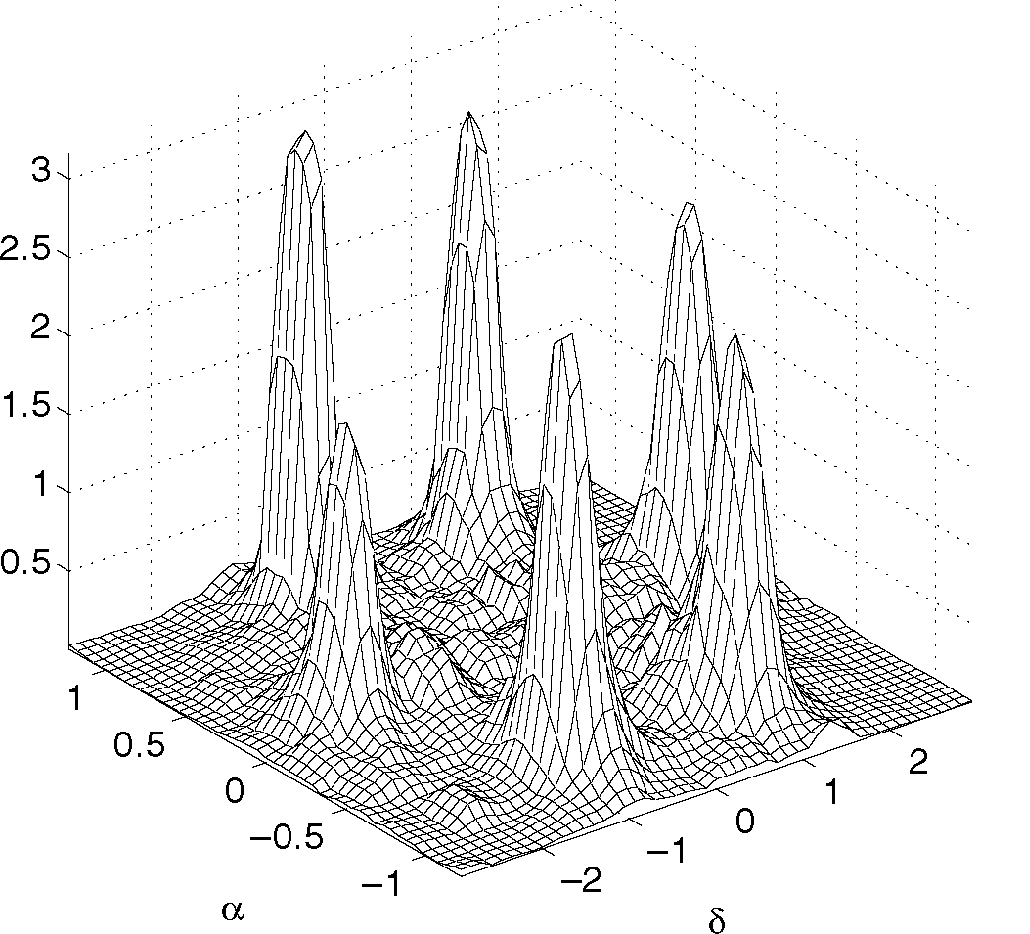
\includegraphics[width = 0.6\linewidth]{./figures/autres/DUET_histogram.png}
\caption{Histogramme 2D pour un signal sonore composé de 5 sources sonores, générant 5 pics \cite{rickard2007duet}.}
\label{fig:DUET_hist}
\end{figure}

Une implémentation de cet algorithme, pour une utilisation en temps réel, est proposée dans \cite{rickard2001real}.
Afin de s'extraire des conditions strictes imposées par la méthode et de s'approcher d'applications plus réelles, \cite{rickard2007duet} propose de considérer l'ajout d'un terme de bruit à l'équation \ref{eq:algo-DUET} et de déterminer l'\textit{atténuation symétrique} $\alpha_j$ et le \textit{déphasage relatif} $\delta_j$ de chaque source :

\begin{equation}
\alpha_j = \frac{\iint_{(\omega,\tau)} \vert X_1(\omega,\tau) X_2(\omega,\tau)\vert ^p \omega^q \alpha(\omega,\tau) d\omega d\tau}{\iint_{(\omega,\tau)}\vert X_1(\omega,\tau) X_2(\omega,\tau)\vert ^p \omega^q d\omega d\tau},
\end{equation}

avec $\alpha(\omega,\tau) = \bigg\vert \frac{X_2(\omega,\tau)}{X_1(\omega,\tau)} \bigg\vert - \bigg\vert  \frac{X_1(\omega,\tau)}{X_2(\omega,\tau)} \bigg\vert$ et

\begin{equation}
\delta_j = \frac{\iint_{(\omega,\tau)} \vert X_1(\omega,\tau) X_2(\omega,\tau)\vert ^p \omega^q \tilde{\delta}(\omega,\tau) d\omega d\tau}{\iint_{(\omega,\tau)}\vert X_1(\omega,\tau) X_2(\omega,\tau)\vert ^p \omega^q d\omega d\tau}.
\end{equation}

Ces deux indicateurs dépendent de deux constantes définies, $p$ et $q$, qui permettent de pondérer le poids de chaque point temps-fréquence :

\begin{itemize}
\item $p$ = 0, $q$ = 0 revient à l'algorithme DUET original,
\item $p$ = 1, $q$ = 0 donne plus de poids à $\alpha_j$ \cite{yilmaz2004blind},
\item $p$ = 1, $q$ = 2 donne plus de poids à $\delta_j$ \cite{yilmaz2004blind},
\item $p$ = 2, $q$ = 2 est adapté aux signaux ayant un faible rapport signal à bruit ou bien pour des mixtures de paroles \cite{melia2007underdetermined}.\\
\end{itemize}

Différentes applications basées sur cet algorithme existent notamment pour des signaux de paroles \cite{yilmaz2004blind, jourjine2000blind}.
Plusieurs développements ont été proposés afin d'étendre l'utilisation de cette méthode. Dans  \cite{melia2007underdetermined} plusieurs versions sont décrites et comparées comme la \textit{echoic DESPRIT} qui propose avec $M$ microphones de retrouver $N$ signaux (en supposant que le nombre de chemins empruntés par les signaux est inférieur à $\sfrac{M}{2}$) ou bien la \textit{echoic ESPRIT}, où il est supposé que le nombre de sources actives simultanément n'excède pas $\sfrac{M}{2}$. \\

\section{Analyse en Composantes Indépendantes}
L'Analyse en Composantes Indépendantes (ACI) \cite{comon_independent_1994, jutten1991blind} est une méthode appartenant aux méthodes dites de \textit{séparation de sources aveugle}, c'est-à-dire qui séparent un ensemble de sources sonores d'une mixture sans (ou avec peu) informations sur celles-ci. L'illustration la plus couramment citée, pour cette méthode, est l'effet \og cocktail party \fg{}. Cet effet résume le processus qui permet à un être humain de séparer la voix de l'interlocuteur, avec qui il discute, du flux sonore environnant composé d'autre discussions, de musique\dots{} Cette capacité est notamment permise par l'indépendance entre le signal \textit{voix} et les autres sources sonores aux alentours ainsi que par l'écoute binaurale du sujet. L'ACI se base sur ces hypothèses et s'exprime alors sous la forme d'un produit matriciel :

\begin{equation}\label{eq:ACI2}
\mathbf{x} = \mathbf{As}
\end{equation}

où $\mathbf{x}$, de dimensions $N \times 1$, exprime l'ensemble des mesures faites par $N$ capteurs, $\mathbf{s}$, de dimensions $N \times 1$, résume les différentes sources présentes et $\mathbf{A}$, de dimensions $N \times N$, une matrice déterministe résumant les aspects de propagation entre les sources et les capteurs.
$\mathbf{A}$ et $\mathbf{s}$ étant inconnus, plusieurs hypothèses sont considérées afin de résoudre le problème : i) $\mathbf{s}$ est composé de sources sonores indépendantes, ii) les sources sonores ne suivent pas de distribution gaussienne (ou pas plus de une), iii), $\mathbf{A}$ est une matrice carrée inversible. Le problème s'exprime alors sous la forme :

\begin{equation}
\mathbf{s} = \mathbf{A}^{-1}\mathbf{x}.
\end{equation}

L'ACI peut être vue comme une extension de l'Analyse en Composante Principale (ACP) où il y est supposé, non pas l'indépendance des composantes, mais leur décorrélation et où sont déterminées les grandeurs qui ont le plus de variances. L'ACI est donc une méthode plus contrainte (des variables indépendantes seront toujours décorrélées alors que l'inverse n'est pas vrai).
De nombreux développements ont été proposés afin d'obtenir une indépendance maximale entre les sources :

\begin{itemize}
\item la minimisation de l'information mutuelle \cite{hyvarinen97independentcomponent} qui consiste à maximiser un calcul de distance (au travers d'une divergence de Kullback-Leibler) entre l'entropie de l'ensemble des composantes et celle d'une composante $i$.
\item La décorrélation non-linéaire qui consiste à minimiser la corrélation entre deux composantes $y_i$ et $y_j$ chacune exprimée par une fonction $f(y)$ et $g(y)$ dont au moins une est non-linaire (polynôme de degré 2 ou plus, fonction tangente hyperbolique\dots). Pour passer de la non-corrélation à l'indépendance, \cite{jutten1991blind} ajoute une condition où la fonction non-linéaire (ou une des deux)  est impaire avec une moyenne nulle.
\item la minimisation de la \og gaussianité \fg{} des composantes, basée sur le \textit{Théorème Centrale Limite} qui démontre que la somme de variables aléatoires indépendantes forme un ensemble gaussien. La recherche de l'indépendance des sources revient alors à minimiser la \og gaussianité \fg{} entre les composantes. Cette approche est la base de la mesure de la négentropie (ou entropie relative) \cite{lee2000unifying} ou de l'algorithme FastICA \cite{hyvarinen1999fast} qui est l'algorithme le plus couramment utilisé pour résoudre l'ACI.
\end{itemize}

Une revue exhaustive des méthodes employées est effectuée dans \cite{hyvarinen2004independent}.
Pour être résolue, l'ACI est, le plus souvent, sur-déterminée, ce qui signifie qu'il y a au moins autant ou plus de signaux captés que de sources sonores. Pour obtenir une matrice $\mathbf{A}$ carrée, une ACP peut être utilisée afin de supprimer les informations redondantes.  Le cas de la sous-détermination a toutefois été étudié, par exemple dans \cite{bofill2000blind} en considérant les signaux comme parcimonieux.
L'ACI a trouvé de nombreuses applications, en tant que méthode de séparation de sources aveugles, dans le domaine médical, pour extraire les différentes composantes d'un signal d'électroencéphalogramme \cite{delorme2007enhanced,makeig1996independent} ou d'une IMR \cite{lee1999independent}, pour traiter des signaux contenant de la parole \cite{sarela2005denoising, hsieh2009independent} ou pour des contenus musicaux \cite{uhle2003extraction, abdallah2003independent}. Des utilisations de l'ACI pour des sons environnementaux existent aussi \cite{lombard2011tdoa, eronen2006audio}. Cette méthode peut également être utilisée pour des antennes acoustiques et pour la formation de voies (\textit{beamforming})\cite{cardoso_blind_1998,saruwatari2003blind}.

La détermination des matrices $\mathbf{A}$ et $\mathbf{s}$ n'est toutefois pas sans générer des ambiguïtés bien identifiées dans la littérature. La première est l'\textit{ambiguïté de permutation} qui traduit la variabilité dans l'ordre de détermination des composantes indépendantes : une composante estimée $s_1$ peut être déterminée à un rang différent sans pour autant changer la reconstruction du signal global. Ce problème est toutefois sans conséquence la plupart du temps. Une seconde limite est l'\textit{ambiguïté d'échelle} qui traduit la possibilité d'avoir un facteur d'échelle présent dans la matrice $\mathbf{A}$ et $\mathbf{s}$ tel que :

\begin{equation}
\begin{bmatrix}
x_{1}\\
\vdots\\
x_{N}
\end{bmatrix} =
\begin{bmatrix}
\alpha_1 a_{11} & \dots & \alpha_1 a_{1N}\\
\vdots & \ddots & \vdots\\
\alpha_N a_{N1} & \dots & \alpha_N a_{NN}
\end{bmatrix}
\times
\begin{bmatrix}
\sfrac{s_{1}}{\alpha_1}\\
\vdots\\
\sfrac{s_{N}}{\alpha_N}
\end{bmatrix}.
\end{equation}

La détermination de l'amplitude exacte des signaux est donc soumise à l'incertitude \cite{naik2011overview}.

\section{Factorisation en Matrices Non-négatives}

La Factorisation en Matrices Non-négatives (abrégée NMF pour \textit{Non-negative Matrix Factorization} en anglais) \cite{lee_learning_1999}, appliquée à l'analyse d'un signal audio-numérique, est une méthode qui est basée sur une représentation linéaire de données :

\begin{equation}
\mathbf{V} \approx  \mathbf{WH}
\end{equation}

où $\mathbf{V}$ est le spectrogramme en amplitude ou en puissance d'un signal audio de dimensions $F \times N$, $\mathbf{W}$ est appelé \textit{dictionnaire} ou \textit{base}. De dimensions $F \times K$, il contient un ensemble de spectres sonores. $\mathbf{H}$, de dimensions $K \times N$ est la matrice d'activation qui traduit les variations dans le temps de chaque spectre de $\mathbf{W}$.  $K$ définit le rang des matrices et est le plus souvent choisi tel que $F\times K + K \times N \ll F \times N$ afin d'être une méthode qui permet la réduction de données.
Là où l'ACI impose une contrainte d'indépendance, la NMF impose celle de la \og non-négativité \fg{} ($\mathbf{V}$, $\mathbf{W}$ et $\mathbf{H} \in \mathbb{R}_+$). Cette contrainte n'autorise alors que des combinaisons additives entre les composantes et leur assure ainsi d'appartenir au même domaine et donc de leur interprétabilité. 
L'approximation entre $\mathbf{V}$ et $\mathbf{WH}$ est résolue en minimisant leur $\beta$-divergence :

\begin{equation}\label{eq:d_v_wh}
\text{min}~D_{\beta}\left(\textbf{V} \vert\vert \textbf{WH}\right) \quad \text{avec} \quad \mathbf{W} \geq 0, \mathbf{H} \geq 0.
\end{equation}

Plusieurs approches existent afin de résoudre le problème \ref{eq:d_v_wh}, basées sur des approches itératives : mises à jour multiplicatives \cite{lee_algorithms_2000}, méthode des moindres carrés alternés \cite{cichocki_regularized_2007}, gradient projeté \cite{lin_projected_2007}\dots{} La NMF permet aussi d'ajouter des contraintes sur chaque matrice \cite{virtanen_monaural_2007, bertin2010enforcing} afin de forcer un type de comportement particulier des matrices suivant le problème posé.

Cette méthode a reçu une grande popularité en trouvant de nombreuses applications pour la musique (transcription de partitions de musique \cite{smaragdis_non-negative_2003,bertin2009tempering}, classification de genre musicaux \cite{panagakis2008music} et d'instruments \cite{benetos2006musical}, séparation des pistes musicales \cite{souviraa2015music}) et pour la parole (débruitage \cite{wilson2008speech,sprechmann2014supervised}, séparation de sources \cite{smaragdis2007convolutive, 
hurmalainen2012detection})\dots{}
Cette méthode a également déjà été confrontée à des sons environnementaux pour différentes tâches comme dans \cite{kumar2016audio} où la NMF est utilisée afin de localiser l'origine de différents extraits sonores. Dans \cite{sobieraj2017masked}, la NMF sert à la détection d'oiseaux dans différents environnements sonores. Dans \cite{heittola_sound_2011}, la NMF est utilisée en vue de détecter plusieurs évènements sonores émis simultanément en représentant les évènements à travers des Chaines de Markov Cachées (HMM) et des Mel Frequency Cepstral Coeffcient (MFCC).  Enfin dans \cite{satoshi_innami_nmf-based_2012}, la NMF est utilisée en tant que méthode de séparation de sources pour extraire différents signaux (voix, aboiement de chien, croassements de grenouille).
Par son fonctionnement, la NMF présente l'avantage, en plus de prendre naturellement en compte le recouvrement temporel entre les sources sonores, d'être adaptée à des réseaux de capteurs monophoniques.

%Emmanuel a fait un travail consequent dans le domaine, as-tu bien cite son travail ?

\section{Détection d'évènements sonores}

Cette approche n'est pas une méthode de séparation de sources puisque l'objectif est d'identifier les sources sonores qui composent une mixture pour ensuite ne considérer que celles d'intérêt.

La reconnaissance et la détection de sources sonores environnementales à l'aide de descripteurs \cite{dufaux2000automatic,defreville_automatic_2006} reçoit une attention croissante. Ces travaux suivent le plus souvent un protocole établi : i) apprentissage d'un détecteur sur une base de données, ii) application de ce détecteur sur une base de test en vue d'estimer les performances de l'outil. Dans \cite{mesaros2010acoustic}, 61 évènements sonores sont détectés parmi des enregistrements audio annotés à l'aide de l'algorithme de Viterbi et des HMM. \cite{ntalampiras2011probabilistic} détecte des évènements anormaux tel que des cris, des tirs d'armes à feu à partir de mixtures sonores synthétisées où le niveau sonore relatif de ces évènements par rapport aux bruits de fond de la scène est échelonné entre -5 dB et 15 dB. Les descripteurs utilisés sont les MFCC, MPEG-7 et les \textit{Perceptual Wavelet Packets} et le classifieur est basé sur un Modèle de Mixtures de Gaussiennes (GMM) et sur des HMM. Ces travaux seront étendus dans \cite{ntalampiras2014universal} pour réaliser un outil de surveillance du trafic routier. Dans le cadre du projet DYNAMAP, un détecteur d'évènements sonores anormaux (DESA) a été réalisé \cite{socoro2017anomalous}. Celui-ci consiste, pour chaque trame temporelle, à y identifier la classe de son principale. Celles qui ne sont pas reconnues comme \textit{trafic} sont alors rejetées et non prises en compte dans l'estimation du niveau sonore du trafic routier. Cet outil se base, là aussi, sur les MFCC (13 bandes), exprimés sur des trames temporelles de 30 ms, couplés à des GMM. Le corpus de test est divisé en deux classes : \textit{urbain} et \textit{banlieue}. Les performances du détecteur, évalué au travers du F-score, est pour chaque classe du corpus de 61,5 $\%$ et de 72,3 $\%$.

\section{Comparaison des approches}\label{part:comparaison_method}

Le Tableau \ref{tab:comparaison_method} compare les différentes caractéristiques requises par l'outil de séparation de sources afin de satisfaire le cahier des charges proposé dans la partie \ref{part:cahier_charges}. Pour rappel, celui-ci doit être adapté aux sons environnementaux présentant du recouvrement temporel et aux réseaux de capteurs monophoniques.

\begin{table}[ht]
\centering
\caption{Comparaison des 4 méthodes de séparation de sources et de la méthode DESA en vue d'estimer le niveau sonore du trafic routier à partir d'enregistrements monophoniques (\og - \fg{} : pas adapté, \og + \fg{} : adapté, \og ++ \fg{} : très adapté).}
\label{tab:comparaison_method}
\begin{tabular}{lcccl}
\toprule
 & \begin{tabular}[c]{@{}c@{}} sons \\ environnementaux\end{tabular} & \begin{tabular}[c]{@{}c@{}}recouvrement \\  temporel\end{tabular} & \begin{tabular}[c]{@{}c@{}} réseau de capteurs\\  monophoniques\end{tabular} &  \\
\midrule
CASA & - & + & - &  \\
\cellcolor[HTML]{C0C0C0}Algorithme DUET & \cellcolor[HTML]{C0C0C0}- & \cellcolor[HTML]{C0C0C0}+ & \cellcolor[HTML]{C0C0C0}- &  \\
ACI & + & ++ & - &  \\
\cellcolor[HTML]{C0C0C0}NMF & \cellcolor[HTML]{C0C0C0}++ & \cellcolor[HTML]{C0C0C0}++ & \cellcolor[HTML]{C0C0C0}++ &  \\
DESA  & ++ & - & ++ & \\
\bottomrule
\end{tabular}
\end{table}


La méthode CASA et l'algorithme DUET sont des méthodes qui sont peu adaptées au cas d'étude présent, car elles sont développées notamment pour des sons harmoniques et qui nécessitent au minimum deux microphones pour chaque point de mesure ce qui n'est pas compatible avec des réseaux de capteurs monophoniques. De plus, basée sur une hypothèse d'anéchoïcité, malgré des extensions pour s'affranchir de celle-ci, la méthode DUET reste peu évidente et adaptée pour un environnement sonore urbain où le champs diffus est prépondérant.
Si l'ACI est utilisé pour des mixtures sonores urbaines, elle l'est pour des antennes de microphones et la formation de voies. Là encore, cette approche n'est donc pas une méthode adaptée à la mise en place de réseaux de capteurs monophoniques. De plus l'\textit{ambiguïté d'échelle} est un frein pour estimer correctement le niveau sonore du trafic. L'outil DESA répond à une grande partie des besoins, mais génère les problèmes classiques de détection  de faux-positifs (des trames contenant des composantes \textit{trafic} mais qui sont identifiées comme \textit{interférante}). De plus, les cas où le trafic et une autre source \textit{interférante} sont présents dans une même trame posent la question de son possible rejet. Ne pas considérer un ensemble de trames où le trafic est pourtant présent (mais rejeté parce qu'elle n'est pas la source principale) peut mener à des estimations du niveau sonore du trafic qui serait sous-estimées. Dans le cas où le trafic est la source sonore principale, aux abords des boulevards ou d'un périphérique, ce problème est limité Mais dans les cas où les rues sont calmes, dans les parcs ou les places où les voix sont plus importantes, même si le trafic est moins présent, sa contribution à l'ESU n'en reste pas moins négligeable et doit être estimée.
Ainsi, c'est donc, la NMF qui, par son fonctionnement (reconstruire le spectrogramme d'un signal audio à l'aide d'un dictionnaire), paraît être la méthode la plus adaptée à ces travaux. 
Celle-ci se base sur un enregistrement audio réalisé par un seul capteur, donc compatible avec les réseaux de capteurs monophoniques. Le recouvrement est naturellement pris en compte par la contrainte de non-négativité qui n'autorise que des combinaisons additives. Ainsi, l'ensemble des sources présentes dans $\mathbf{W}$ peuvent être, pour une trame donnée, toutes considérées simultanément. Enfin, son application à des sons environnementaux dans de précédentes études, même si le trafic n'en est pas la source sonore principale, permet d'assurer la compatibilité de cette méthode face à des mixtures sonores urbaines.